\chapter{Application}\label{app}
This chapter describes how browser extensions are built in the Google Chrome web browser, focusing on architecture and security features. Browser extensions can be utilized to build an application implementing the \emph{HCP scheme} as described in \autoref{ch:hcp}. The scheme is different from other traditional password managers since it does not \emph{store} the password, but the challenges \emph{help} the user to remember strong passwords. The idea by using browser extensions to implement this is to have an extension monitor the password fields of the sites a user visits and update the challenges depending on the current state of the active site. This technique is described and a prototype extension demonstrated. 
\section{Browser Extensions}\label{browser-extensions}
Modern computer users shift towards doing more and more work through their web browsers. Web applications have become popular due to the ubiquity of browsers, thus allowing web apps to run anywhere. A web app can run on any platform running a web browser. Updates can be applied quickly without having to distribute patches to a possibly huge amount of devices.
\par Browser extensions add additional features to the web browser allowing users to tweak the experience of the web pages visited. Typical examples are extensions adding to, or tweaking already present features of the browser such as changing how bookmarks are managed, or adding additional features such as blocking advertisements. Lately browser extensions have been extended even further allowing standalone applications to be developed running as native applications \footnote{A new breed of Chrome apps - \url{http://chrome.blogspot.no/2013/09/a-new-breed-of-chrome-apps.html} - accessed: 2015-03-02}. This allow developers to create desktop apps using the same technology as in web apps, mainly HMTL5, Javascript and CCS.
\par This section presents Google Chrome browser extensions, including architecture and security mechanisms.

%This project will utilize chrome extensions to create a password manager running in the browser. 
%The user interface will be in a panel spawned by a browser action activated when the user click the icon in the navbar. 
%The user interface is built using the open-source web application framework AngularJS \cite{angularjs}, storage is done using the chrome local storage API.

\subsection{Extension Security}\label{extension-sec}
\par Browser extensions introduce some security concerns which must not be forgotten while developing applications using this environment. Chrome extensions run in the browser with access to both the DOM (Document Object Model) of the active page as well as the native file system and connected devices. The overall architecture of a Chrome extension is summarized in \autoref{extension-architecture} and described in the chrome extension documentation\footnote{What are extensions? - \url{https://developer.chrome.com/extensions/overview} - accessed 2015-03-02}. This section describes the architecture considering security concerns relevant when developing chrome extensions which handle sensitive data such as passwords.

%The extension core consist of the actual application interface visible to the user as well as long running background jobs and business logic. The background page can be used to spawn panels or popups, and has access to browser APIs.  The extensions is activated through a icon in the browser navbar as seen in \autoref{extension-ux}. Clicking the icon typically spawns a popup or a panel to interact with the user. In addition to the core, each extensions can have content scripts which has access to the content of the current active web page, and can monitor and alter \gls{dom} of this. 


\begin{figure}[ht]
   \fbox{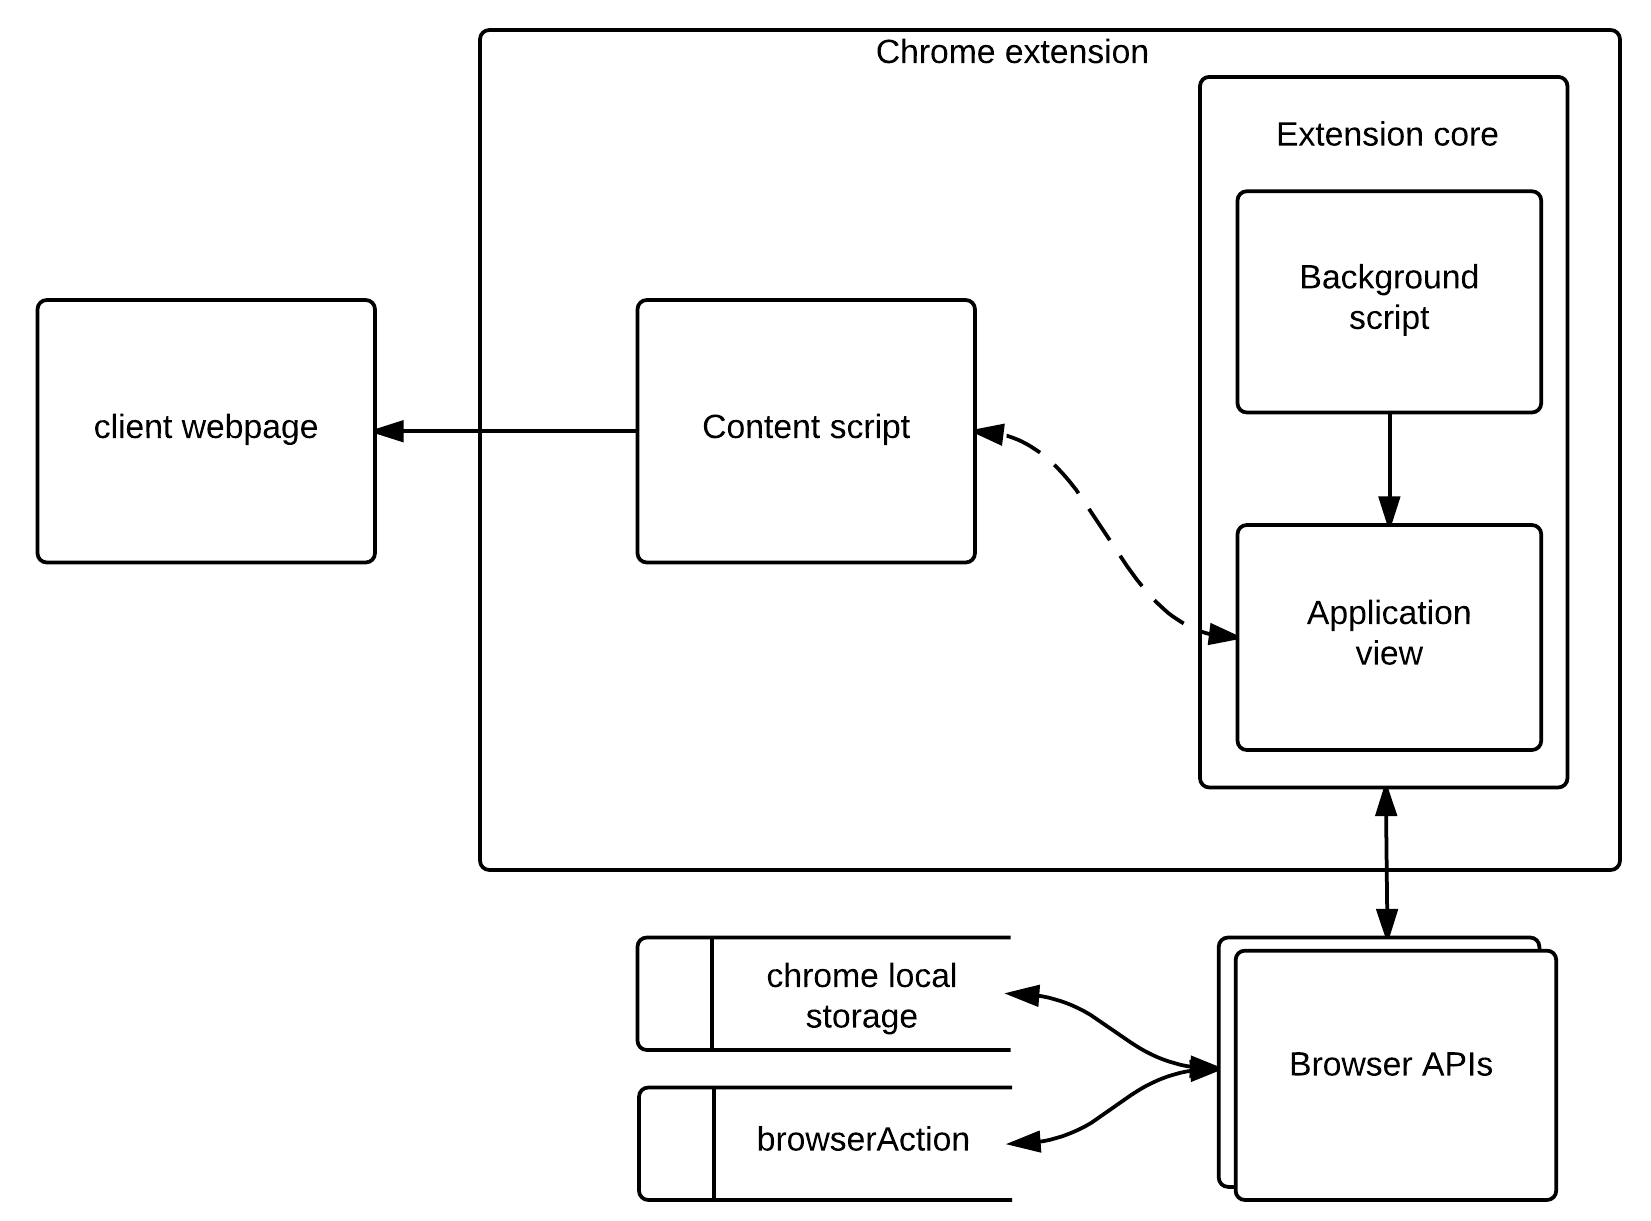
\includegraphics[width=\textwidth]{chrome-extension-architecture} }
    \caption{Chrome extension architecture.}
    \label{extension-architecture}
\end{figure}

\par Earlier extensions written for IE and Firefox ran in the same process as the browser and shared the same privileges. This made extensions an attractive entry point for attackers, since a buggy extension could leave security holes leaking sensitive information or even provide an entry point to the underlying operating system. For these browsers several frameworks for security have been proposed \cite{firefox-ie, js-info-flow}, trying to mitigate vulnerabilities is browser extensions. 
\par The Chrome extensions architecture is built from scratch with security in mind. Chrome uses a permission system following three principles \cite{liu-chrome}; \emph{least privileges}, \emph{privilege separation} and \emph{process isolation}. 

\paragraph{Least privilege} specifies that extensions should only have the privileges they need to function, not share those of the browser. The privileges of each extension are requested in the \emph{manifest} file\footnote{Manifest file format - \url{https://developer.chrome.com/apps/manifest} - accessed 2015-03-04}. This json file needs to be included in all Chrome extensions, and consist of all the permissions needed by the extension as well as some meta data and version information. This is done to prevent compromised extensions from exploiting other permissions than those available at runtime. An example of a manifest file can look like this: 

\begin{verbatim}
{
    "name": "Example extensions",
    "description": "An example extensions to demonstrate how the
                    manifest file works.",
    "version": "1.2",
    "manifest_version": "2"
    "background_page": "main.hmtl",
    "permissions": [
        "bookmarks",
        "storage",
        "https://*.ntnu.no"
    ]
}
\end{verbatim}
This extension has specified access to the bookmarks API, Chrome local storage and all sub domains of ntnu.no. Extensions can request different permissions in the manifest file including web site access, API access and native messaging. If an extension contains weaknesses it will not compromise any other parts of the system not covered by the specified privileges. For the least privileges approach to work properly each developer should only request the permissions needed. Barth et al. \cite{protecting-browsers} examined this behavior and concluded that developers of Chrome extensions usually limit the origins requested to the ones needed. 

\paragraph{Privilege separation.} Chrome extensions are, as mentioned, divided into components; content scripts, extension core and native binaries. The addition of native binaries allows extensions to run arbitrary code on the host computer, thus posing a serious security threat. This project does not use this permission, and does not have the accompanying problems neither. 
\par \emph{Content scripts} are Javascript files allowing extensions to communicate with untrusted web content of the active web page. These scripts are instantiated for each visited web page and has direct access to the DOM of these, allowing both monitoring and editing of DOM elements. To be able to inject content scripts to a visited page, the origin of the site has to be added to the manifest file. Other than this permission, content script are only allowed to communicate with the extension core. It is important that the privileges of these scripts are at the minimum level since they are at high risk of being attacked by malicious web sites \cite{chrome-extension-dangers}, due to the direct interaction with the DOM. 
\par The \emph{extension core} is the application interface responsible for interaction with the user as well as long running background jobs and business logic. The core is written in HTML and Javascript and is responsible for spawning popups and panels, as well as listening for browser action. The typical way to activate an extension is by clicking an icon in the navigation bar, which then activates either a popup or a detached panel. The core is the component with the most privileges as it does not interact with any insecure content directly, only through direct messaging to a content script or using http requests if the target origin is defined in the manifest. 
\par In addition to this, the core has access to the extension APIs, these are special-purpose interfaces providing additional features such as alarms, bookmarks, cookie and file storage. The APIs are made available through the manifest file and only those specified there can be used. \autoref{extension-ux} illustrates the interaction between the background page, content scripts, panels and active web page. The information flow starts by clicking the extension's icon in the navigation bar which launches the background page spawning a panel in the browser. A content script is injected in the current web site (google.no in the example), the script now have access to the DOM of this site and can communicate with the background which in turn can update the panel. 


\begin{figure}[ht]
    \fbox{ 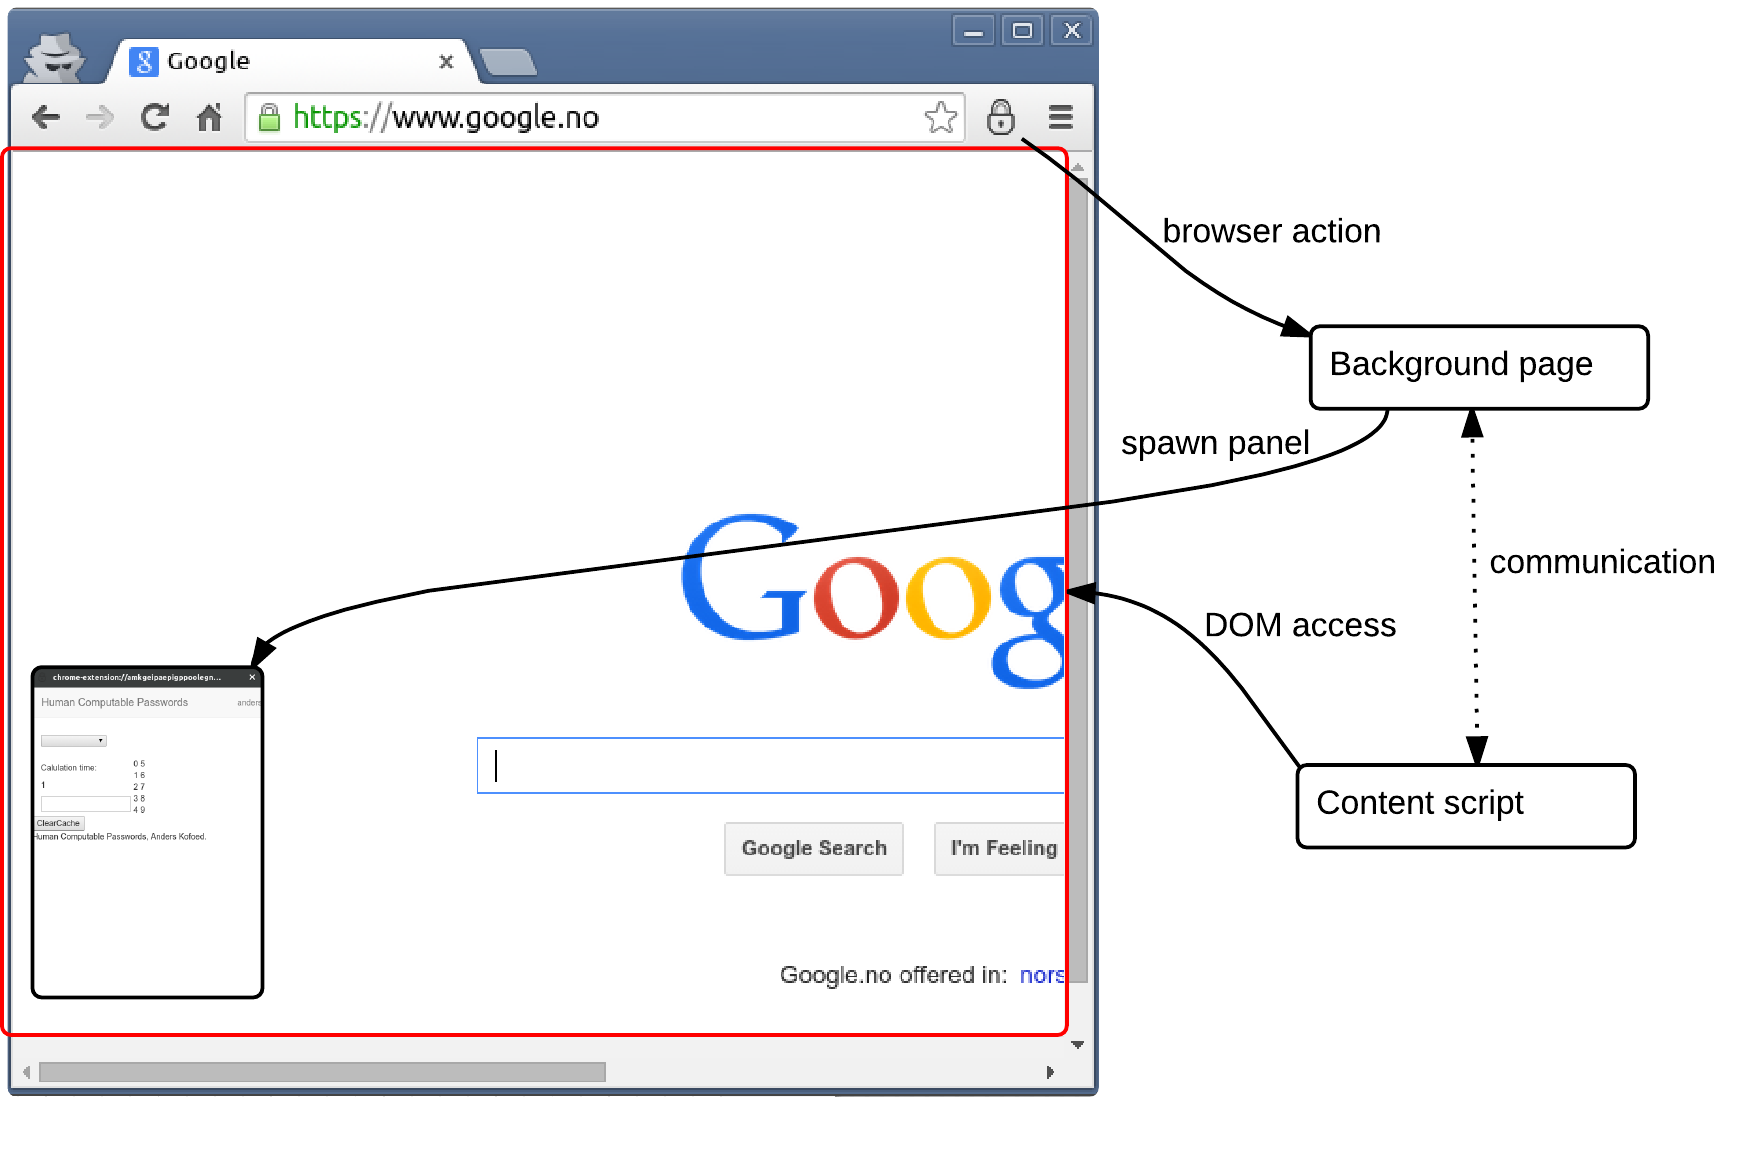
\includegraphics[width=\textwidth]{chrome-extension-ux} }
    \caption{Chrome extensions browser action and content scripts.}
    \label{extension-ux}
\end{figure}

\paragraph{Process isolation} is a set of mechanisms shielding the component from each other and from the web. Usually when Javascript is loaded from the web the authority of the script is limited to the origin from where the script is loaded \cite{protecting-browsers}. Since the scripts used by the extensions are loaded from the file system, they do not have an origin in the same sense, and thus need to be assigned one. This is done by including a public key in the url of the extension, allowing a packaged extension to sign itself, freeing it from any naming authority or similar. The public key also enables usage of persistent data storage, since the origin of the extension can stay the same throughout updates and patches. This would not be possible otherwise since the Chrome local storage API relies on origin. Each extension has a private/public key pair, a hash of the public key is used as ID and each updated version uploaded will be sign with the private key. By doing this the ID stays the same throughout versions and can be verified by when uploading and by Chrome storage after releasing a new version. 


\par The different components also run in different processes. The content scripts are injected and ran in the same process as the active web page, while the core run in its own process started when the extension is initiated. This protects against Javascript injections from malicious web sites\cite{javascript-injection}. Since the content script executes in the same environment as the active web page, users may visit websites hosting content meant to exploit extensions\cite{carlini-chrome}, possibly stealing sensitive information or issue fake requests.
\par Finally content scripts are ran in a separate Javascript environment isolating it from the possibly insecure environment of the web site. The environment of the content scripts are called isolated world, which in practice is a separate set of Javascript objects reflecting the ones of the underlying DOM of the web page. This means that the content script can read and edit the DOM of the page it is injected into, but not access variables or Javascript functions present in the web page. Both the page and the content scripts sees no other Javascript executing in their own isolated world, but they share the same DOM\footnote{Content Scripts - \url{https://developer.chrome.com/extensions/content_scripts} - accessed: 2015-03-05}.


\section{Human Computable Passwords Chrome Extension}
Chrome extensions are very useful in that they can be run from any computer with Google Chrome installed, thus on any operating system and on any computer. An extension makes it possible to run applications while browsing the web, which in the case of a password management scheme is very useful. An application meant to help the user recall complex passwords should preferably be visible simultaneously with the password field. Popular password management software today are usually web applications, mobile applications or native desktop applications\footnote{Five Best Password Managers - \url{ http://lifehacker.com/5529133/five-best-password-managers }}, some of these might include plug-ins in from of browser extensions. All of these password managers are reliably storing all the passwords as described in \autoref{subsec:pms}, then they are either auto-filled into the login fields or through copy pasting manually, which introduce several security issues \cite{protecting-browsers, javascript-injection, chrome-extension-dangers, carlini-chrome, liu-chrome, pw-managment-attacks}
\par This section presents the design and prototype implementation of the HCP scheme as presented in \autoref{ch:hcp}. The design evolves around the fact that the scheme does not have to store anything securely, though it is important to make it as easy as possible for the user. The architecture is similar to the one explained in \autoref{browser-extensions} using content scripts to monitor the password fields of the active browser session. The user interface is presented through a ``panel'' in the browser. Panels are windows that stay in focus while interacting with other windows or applications \footnote{"Panels"- The Chromium Project. \url{https://www.chromium.org/developers/design-documents/extensions/proposed-changes/apis-under-development/panels}}.


The application implementing the HCP scheme is an extension helping users with storage and management of challenges for their accounts. The generation of secret mappings is not part of the application, this should be done through a separate program on the user's local computer. Such a program would follow algorithm \ref{gen-mapping}. The requirements and key components of the design are described next.



\subsection{System Requirements.}
\begin{itemize}
    \item Provide users interface making it easy for the user to calculate their password.
    \item The application should keep track of the active site, displaying challenges for the correct site without user interaction.
    \item Add new sites to the system easily. 
    \item The displayed challenge should update seamlessly while typing the password.
    \item Users should be able to type their passwords directly in the password field of the active site.
    \item When adding a new site to the system, users should be able to classify the account(see \autoref{classification}), affecting the number of single digit challenges created.
\end{itemize}



\subsection{Key Components}

\subsubsection{AngularJS.} The front-end is built and updated using AngularJS\footnote{AngularJS - \url{https://angularjs.org/}}, which is an open source, client-side Javascript framework. Angular is built using a variation of the model-view-controller architecture \cite{mvc}, though the creators of Angular state that Angular is a model-view-whatever framework\footnote{Model-View-Whatever - \url{ https://plus.google.com/+AngularJS/posts/aZNVhj355G2 }}, the point being that what the architecture is called is not important. 
\par The \emph{view}s in Angular are templates written entirely in HTML, making it easy to read and update. The \emph{controller} contains all the business logic used by the view. The views and controllers are connected using a shared object called \emph{\$scope}, variables or functions on this object is usually defined in the controller and accessed by the view using double curly brackets (e.g. \{\{name\}\} to access the name variable on \emph{\$scope}). Figure \ref{angular-data-binding} shows how scope is used to share variables between the controller and the view. 
See "Angular Essentials - Rodrigo Branas"\cite{angularjs-book} for a step-by-step introduction to AngularJS.

\begin{figure}[ht]
    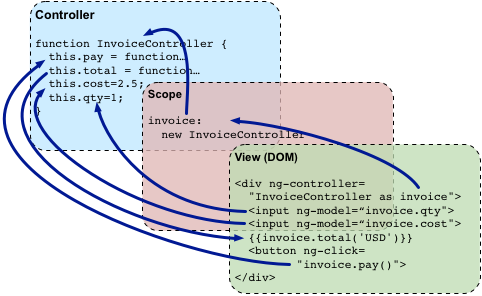
\includegraphics[width=\textwidth]{angular-data-binding} 
    \caption{Angular data binding with controller, view and scope. Figure from AngularJs developer guide.}
    \label{angular-data-binding}
\end{figure}


\par The main benefits of using Angular in this project is the data-binding which makes it easy to update the HTML shown to the user. The extension takes advantage of this when updating the challenges seamlessly while the user calculates his password. The content of the extension changes according to the data filled in the password field without reloading the extension. 

\subsubsection{Chrome Storage.}\label{chrome-storage}
\emph{Local storage\footnote{Local storage - \url{ http://diveintohtml5.info/storage.html }}} is a way for applications to store data persistently and securely in the browser of clients. It is meant as an improvement of cookies which is the usual way of storing user data across sessions. The biggest problem with cookies is that they are sent with every HTTP request and thus slow down the applications using them. Local storage allows applications to store (key, value)-pairs in the browser. 
\par \emph{Chrome storage}\footnote{chrome.storage - \url{https://developer.chrome.com/extensions/storage}} is close to the same as local storage, differences being that Chrome local storage allows applications to store data in what is called ``chrome.storage.sync''. This specific storage saves data locally, but also syncs it with the currently active Chrome account, allowing users to log into their accounts in any chrome browser and access the same application data. Chrome storage also allows storage of objects compared to local storage which only allows storing strings. This project is using Chrome storage to persistently store challenges across sessions, and also provide backup. This way each user is able to keep challenges for all their accounts within the storage of their Google account. This is a important feature since it allows access to the challenges from remote locations as well.

\subsubsection{Content Scripts.}\label{cs}
Content scripts are Javascript files running in the context of the active web page, as browsed by the user. These scripts have direct access to the content of the active site and can thus monitor and attach event listeners to the content of the page. The content scripts are isolated from the extension itself as describe in \autoref{extension-sec}, thus protecting the extension from possibly harmful sites trying to exploit weaknesses in the content script. Because of this the content scripts has to communicate with the extension through Google Chrome's built-in message passing system. Chrome message passing\footnote{Chrome message passing - \url{https://developer.chrome.com/extensions/messaging}} allows scripts to listen for and respond to messages. One side sets up an event listener listening for messages, when a message is sent from the other side this event triggers and the message can be received and parsed. 
\par The content scripts and the message passing system are likely points of attack for adversaries. The content script can monitor the value of the password field and thus, in theory, steal passwords if a malicious script was able to trick it into leaking them. The communication channel is not particularly prone to attacks since even if an adversary eavesdropped all data sent on it, the only information leaked would be the current length of the password. It is though important that the design is like this since the mistake of sending the whole password string, which might seem like a solution, would be potentially dangerous. 
\par Typical usage of content scripts in this application is to attach event listeners to the password fields of the pages visited by users, and message the extension when the value of the password field changes. When a change happens, the content script sends a message containing the current length of the typed password, so that the extension can display the correct challenge. In example if the user has entered 4 characters of his password the extension should display the 5th challenge etc. The content script also keeps the extension updated on the URL of the current page, by sending a message every time a page is loaded. The extension then displays the challenges corresponding to the password of that site. If the site does not have challenges stored by the application, users can generate new ones and store these in the system through clicking a button.  

\subsection{User interface}
The user interface is very simple, two possible screens are displayed to the user. Either, challenges associated with the current active page, or a dialog asking users to generate new challenges. When adding a new site, users are asked to categorize the site as low, medium or highly sensitive. Depending on this choice a set amount of challenges are generated and stored. The most important feature of the user interface is that it automatically updates depending on what site the user is currently browsing, and displays the correct challenge while typing passwords. Wireframes illustrating the page schematics of the extension are shown in figures \ref{add-new-screen} and \ref{challenge-screen}. 

\begin{figure}[ht]
    \centering
    \begin{subfigure}[t]{0.45\textwidth}
        \centering
        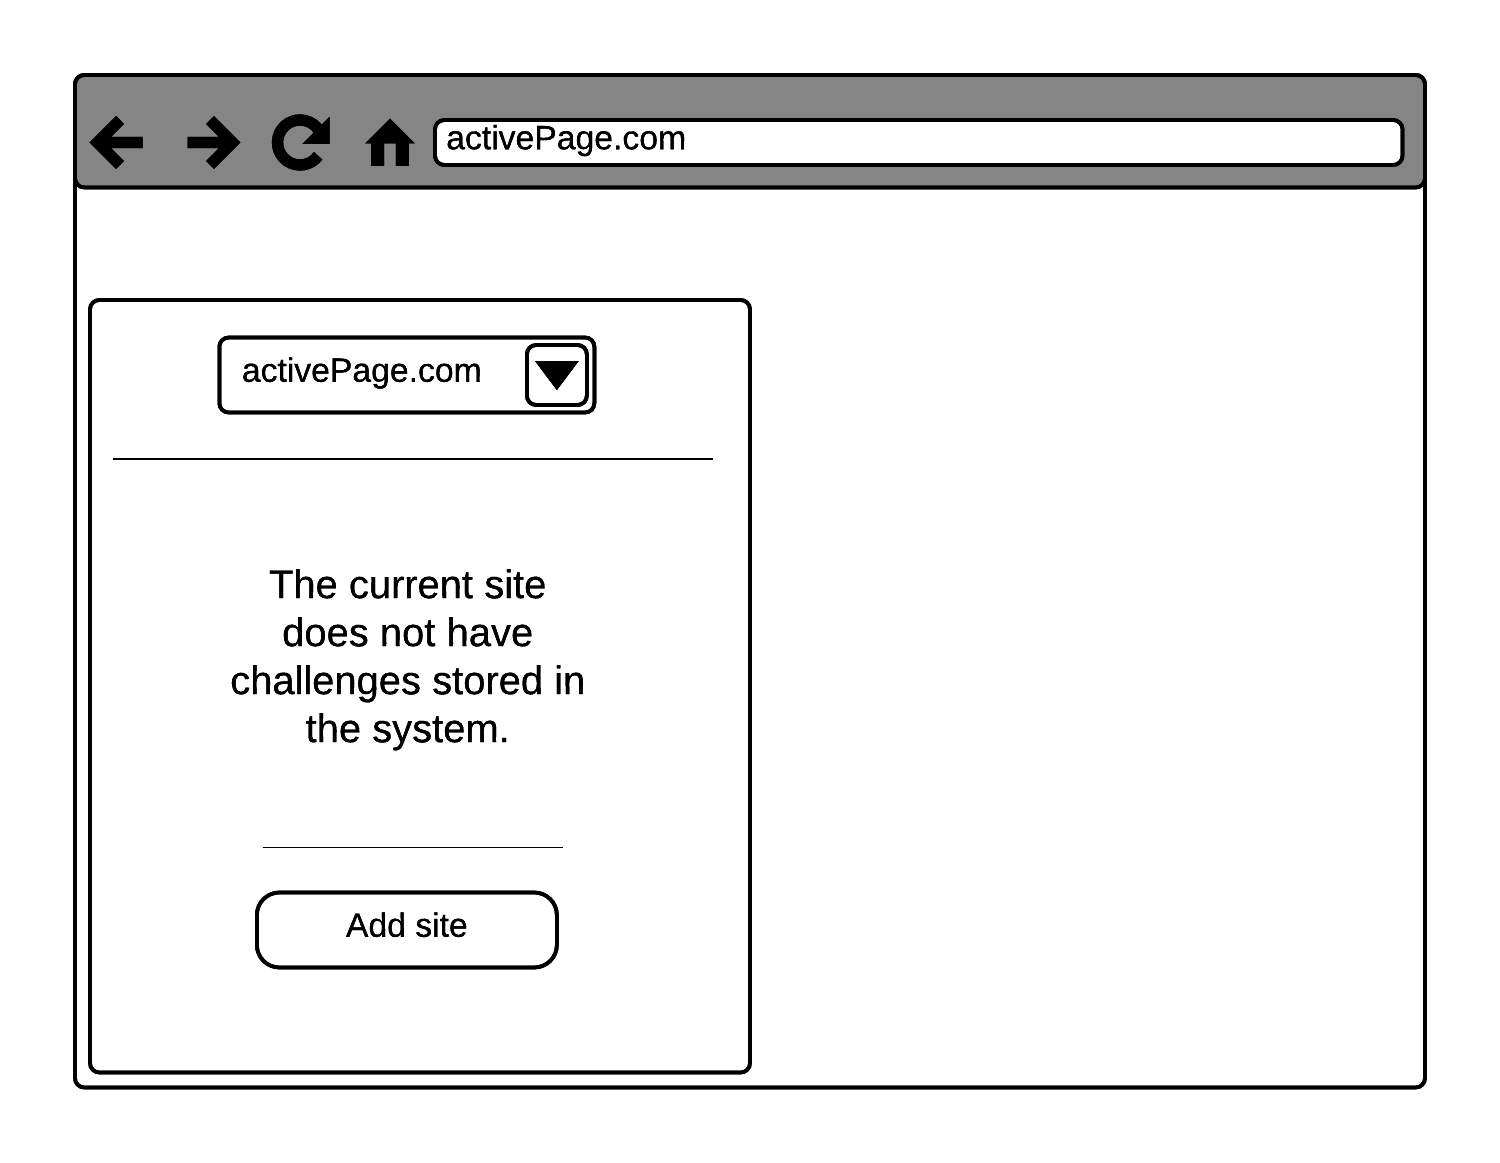
\includegraphics[width=\textwidth]{wireframe} 
        \caption{Screen seen by the user when launching the extension while visiting a page that is not stored in the system.}
        \label{add-new-screen}
    \end{subfigure}
    \hfill
    \begin{subfigure}[t]{0.45\textwidth}
        \centering
        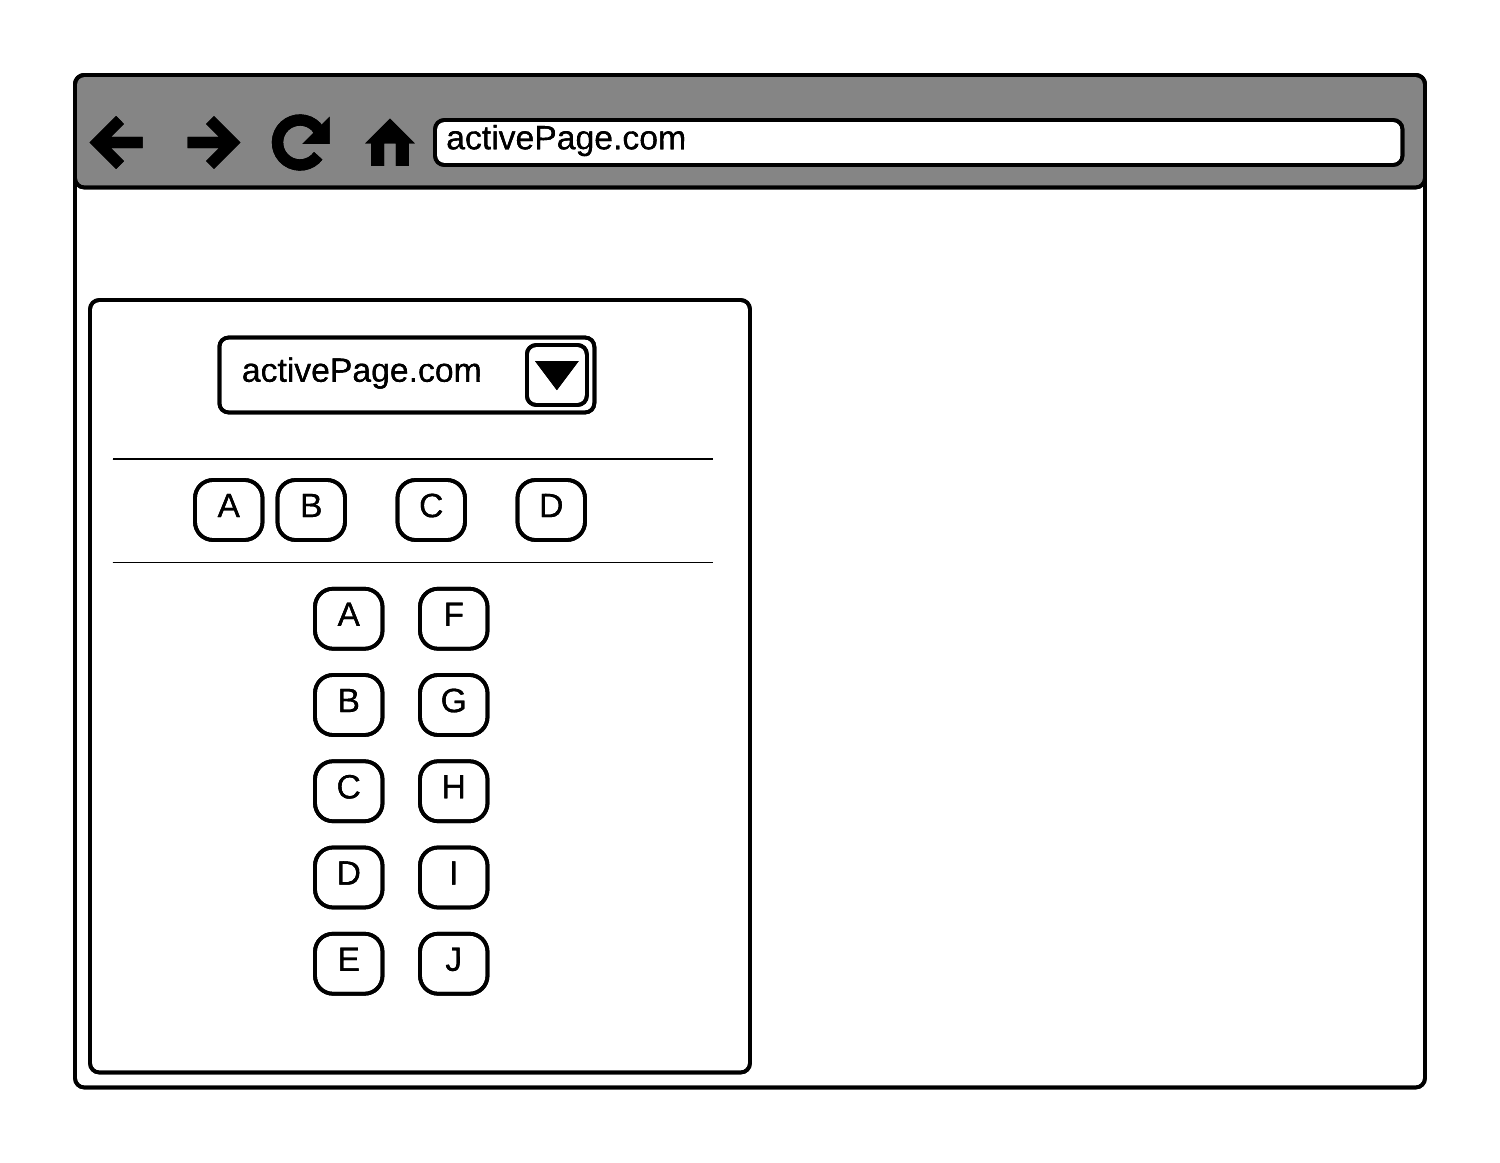
\includegraphics[width=\textwidth]{wireframe2} 
        \caption{Screen seen by the user when loading a site with challenges stored in the system. }
        \label{challenge-screen}
    \end{subfigure}
    \caption{Wireframes illustrating the page schematics of the extension.}
    \label{wireframes}
\end{figure}

\subsection{Implementation}
The implementation follows the design described in the previous section, this section describes how the extension is implemented and demonstrates the actual application in action. 


\par \autoref{class-diagram} shows the complete architecture of the system.
 The content script attaches an event listener to the password field of the active site. If the content of the password field changes, the script sends a message using Chrome message passing containing the current length of the password. The controller receives the new password length from the content script, and updates the challenges displayed. When users visit a new site, the URL is sent to the controller, which then updates the view with new challenges associated with that site.

\begin{figure}[ht]
    \centering
    \fbox{ 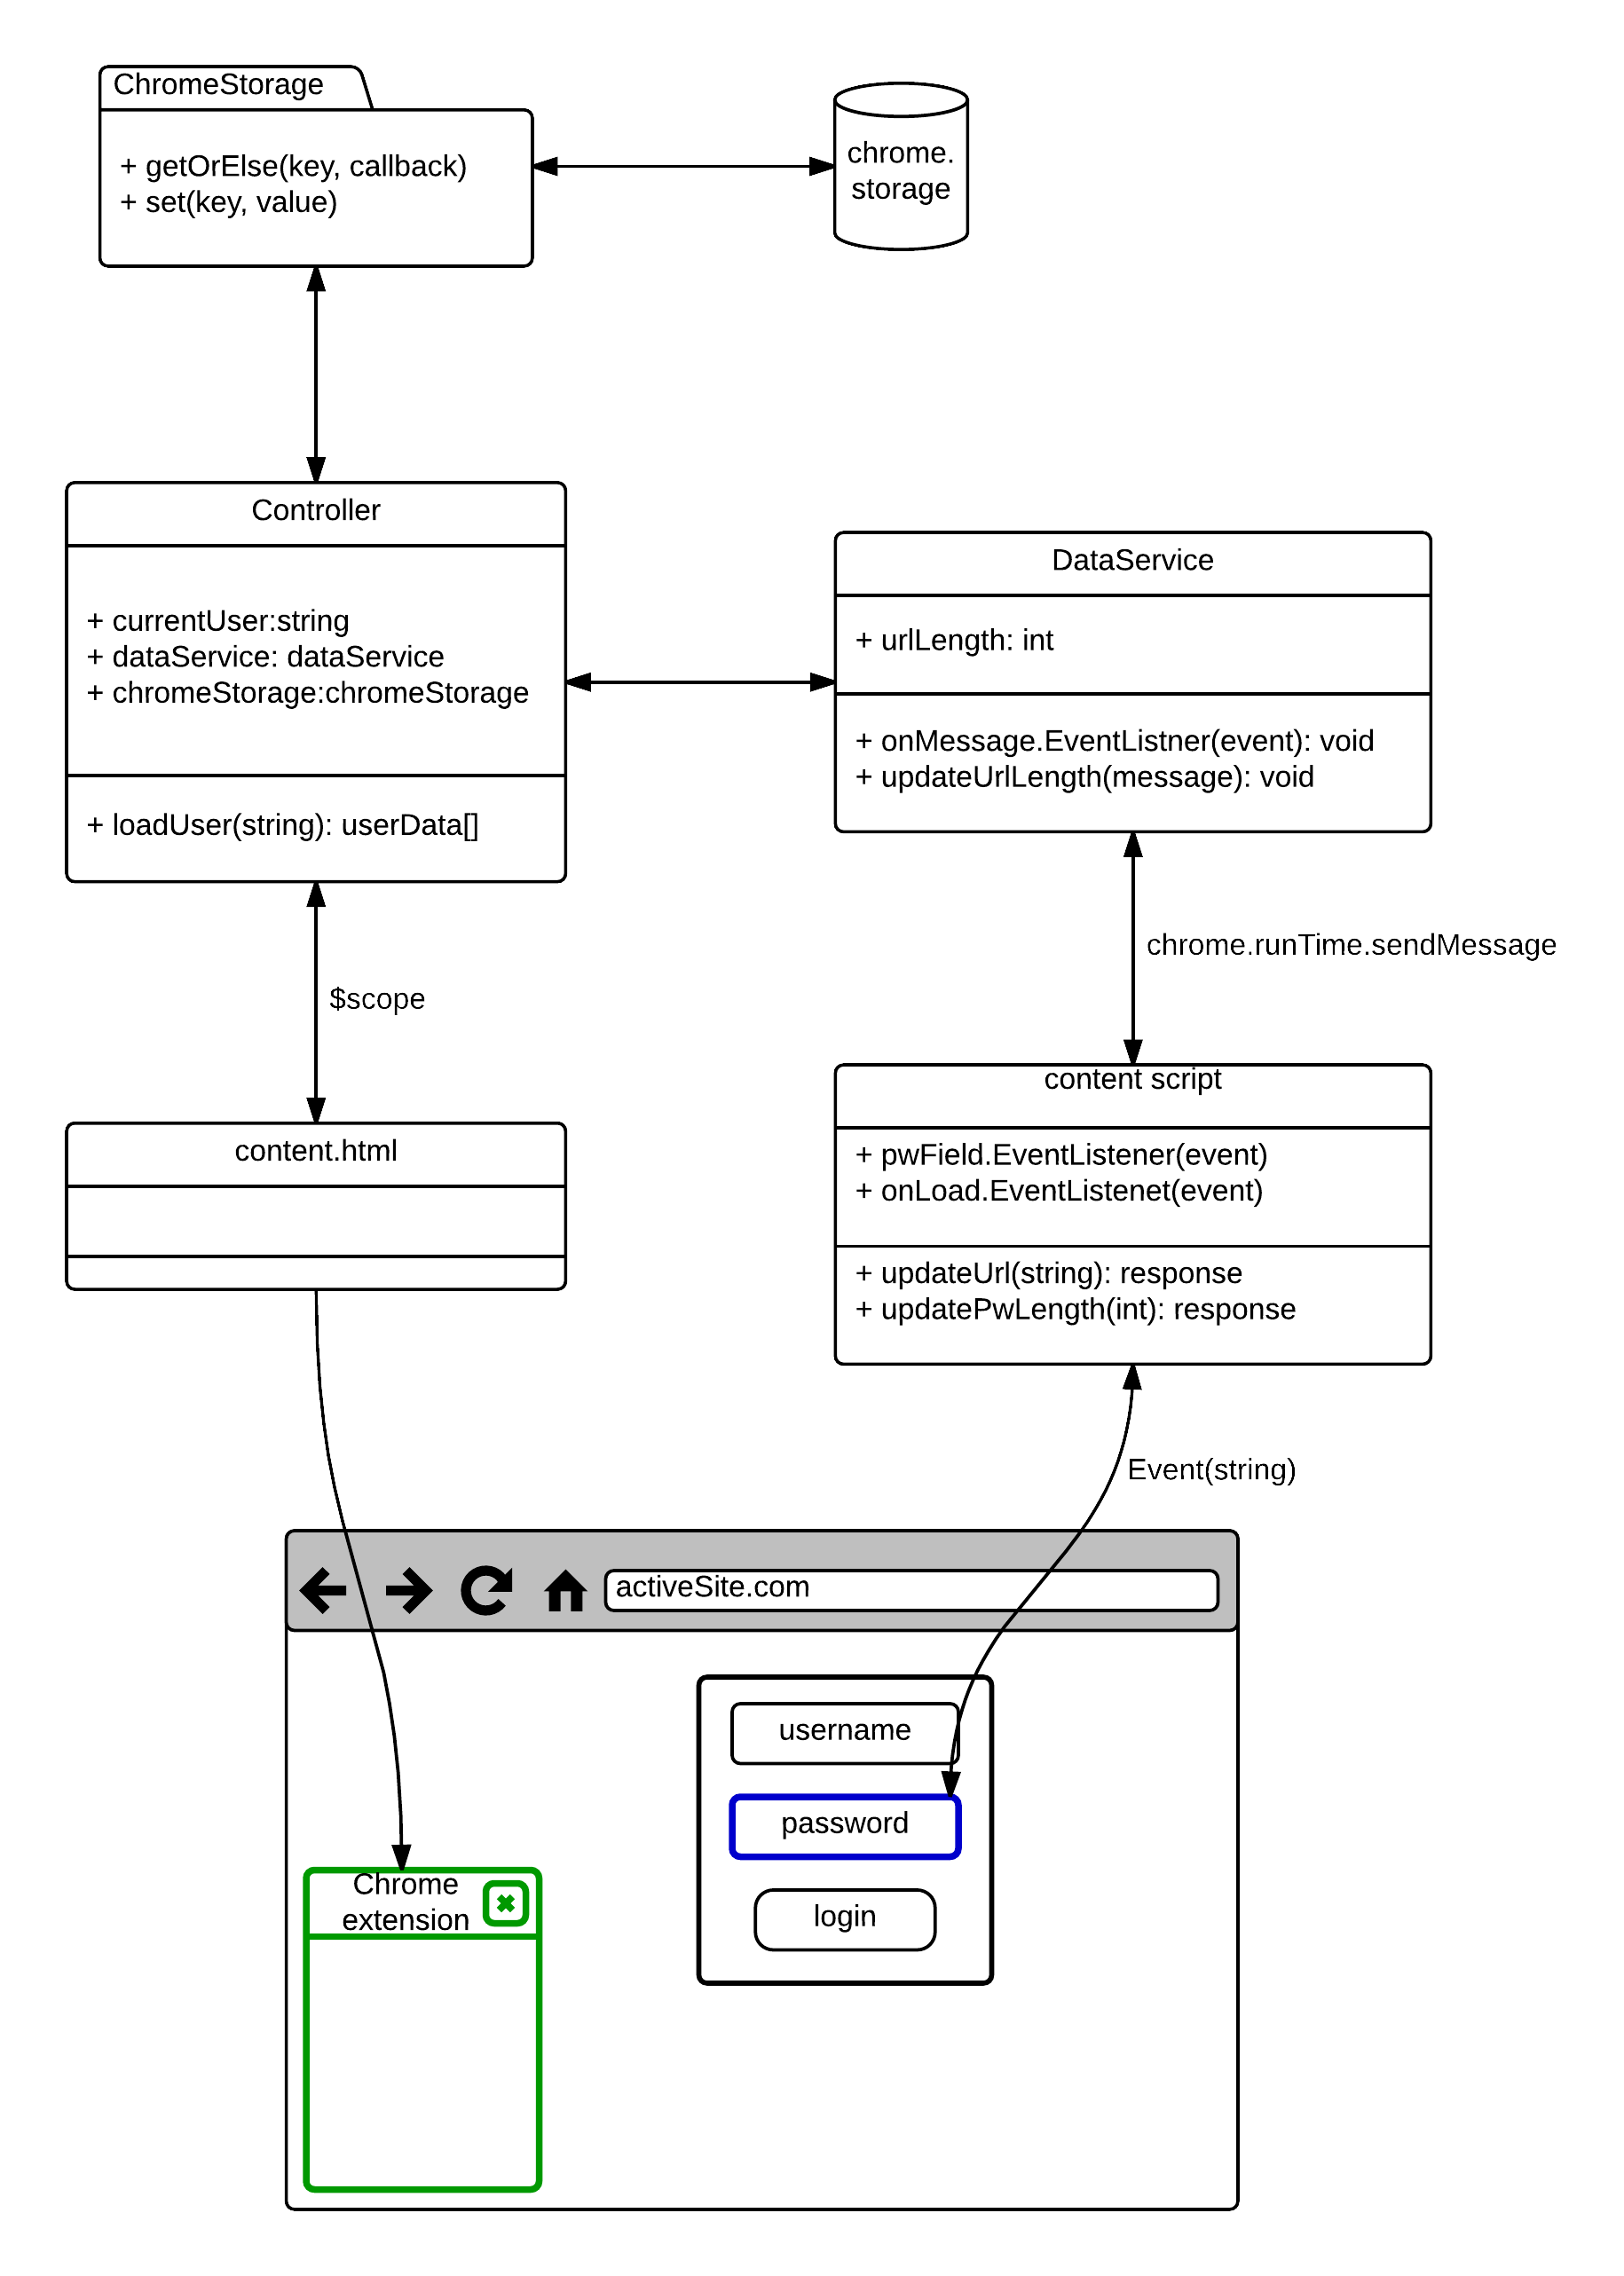
\includegraphics[width=0.9\textwidth]{class-diagram} }
    \caption{Class diagram of the HCP Chrome extension.}
    \label{class-diagram}
\end{figure}

\par The classes seen in figure \ref{class-diagram} are all represented in the implemented version of the extension. The construction and responsibilities of the classes are summarized in the following list. The code of the implementation for each component is explained in more detail in appendix \ref{extension-classes}.

\begin{itemize}
    \item \textbf{Controller} is responsible for the business logic related to the information shown to the users in the extension. The controller first tries to load the user data stored in Chrome storage, if no user has been created, typically if it is the first time the extension is loaded, a new user is created. The controller keeps track of the URL of the current active page and the current length of the password field. It listens for messages from the content scripts and updates the URL and password length variables with the info received. The controller class used in the extension is described in appendix \ref{app:controller}.
    \item \textbf{ChromeStorage\footnote{angular-chrome-storage - \url{https://github.com/infomofo/angular-chrome-storage}}} is a utility resource used to access Chrome local storage (see \autoref{chrome-storage}). This module is essentially a wrapper making it easier to retrieve data from Chrome storage, while also providing useful debugging and cache management functions.
    \item \textbf{Content script} is responsible for attaching event listeners to the password field of the currently active page.. It also listens to the onload event\footnote{Event triggered when a new page is loaded in the browser.}, sending URL updates to the controller every time a new page is loaded. The content script of the extension built in this project can be seen appendix \ref{app:content-script}.
    \item \textbf{main.html} is the view of the application, responsible for the user interface. The view receives updates from the controller through the \$scope variable. When the controller updates in example the current password length, this is reflected in the view where different objects are shown. If the current URL is not in the user's list of saved sites, the view shows a dialog allowing the user to add it. When adding a new site the user should update the password of that site by calculating the response to the challenges. A snippet of the view is shown in appendix \ref{app:view}. 
    \item \textbf{app.js} is the focal point of the application, responsible for initializing the Angular app and routing of views. In this project this file also includes some helper functions which can be seen in appendix \ref{app:app.js}.
\end{itemize}

\paragraph{Random numbers} are an important component of the application since all the security relies on the fact that the secret mapping and the challenges are chosen at random. As for this application, the only concern is the challenges, since the secret mapping would be generated using a separate program on each client's machines. Javascript provide a function called \emph{Math.random} which is not considered cryptographically secure~\cite{js-crypto} and should thus not be used. New browsers now support a new method which are considered to be the best suited random source for cryptographic purposes, the method is called \emph{window.crypto.getRandomValues()}\footnote{RandomSource.getRandomValues() - \url{https://developer.mozilla.org/en-US/docs/Web/API/RandomSource/getRandomValues}}. The application uses this function as the source of randomness to generate challenges. The random number generator used can be seen in appendix \ref{app:app.js}.

\paragraph{Mapping objects.} The application as implemented and demonstrated in this chapter uses the alphabet as mapping objects. As explained in \autoref{ch:hcp}, these objects could be anything and are fixed in this presentation for simplicity. There is a folder in the implementation where all the pictures are kept, these could easily be exchanged with other pictures to better suite the user. 

\paragraph{Launching} the application is done by clicking an icon in the browser toolbar which launches the extension in a panel floating on top of the other browser windows and tabs. This behavior is specified in the \emph{background page\footnote{Background pages - \url{https://developer.chrome.com/extensions/background_pages}}}. The background page is the ``launcher'' of the extension, it waits for users to click the extension icon, firing a browser action event. On catching this event, the script spawns a panel, with the Angular application as content. \autoref{background} shows the background page of this extension. After spawning the panel, the background page is standby doing nothing, everything now happens through the Angular application running inside the panel. 

\lstinputlisting[caption=Background page., label=background, style=jsStyle, basicstyle=\small, frame=single]{code/background.js}

\subsection{Demonstration}\label{demo}
After launching the extension, as previously explained, users are presented with the window shown in figure \ref{launch-screen}. In this example the active site does not have a record in the user's challenge database, thus the ``add new'' dialog. By clicking the button, new challenges are generated and stored in the database as a new site. The site is automatically added with the current site domain as key together with randomly generated challenges. Before adding the site, users can specify which category they rate the site in (low, medium or high), depending on this choice, 5, 10 or 15 challenges are generated. Next time the user visits the same page, challenges will appear. After adding a new site, it is the users responsibility to change the password of this site so it matches the challenges.

\par Figures \ref{ch-screens}a-d shows how a user would use the extension when logging in to a site. When launching it, the system receives the current sites domain and loads the first challenge associated wit that site. The user then calculates the first character using the challenges displayed. When this is entered in the password field, new challenges appear until the whole password is calculated. 

\begin{figure}
    \centering
    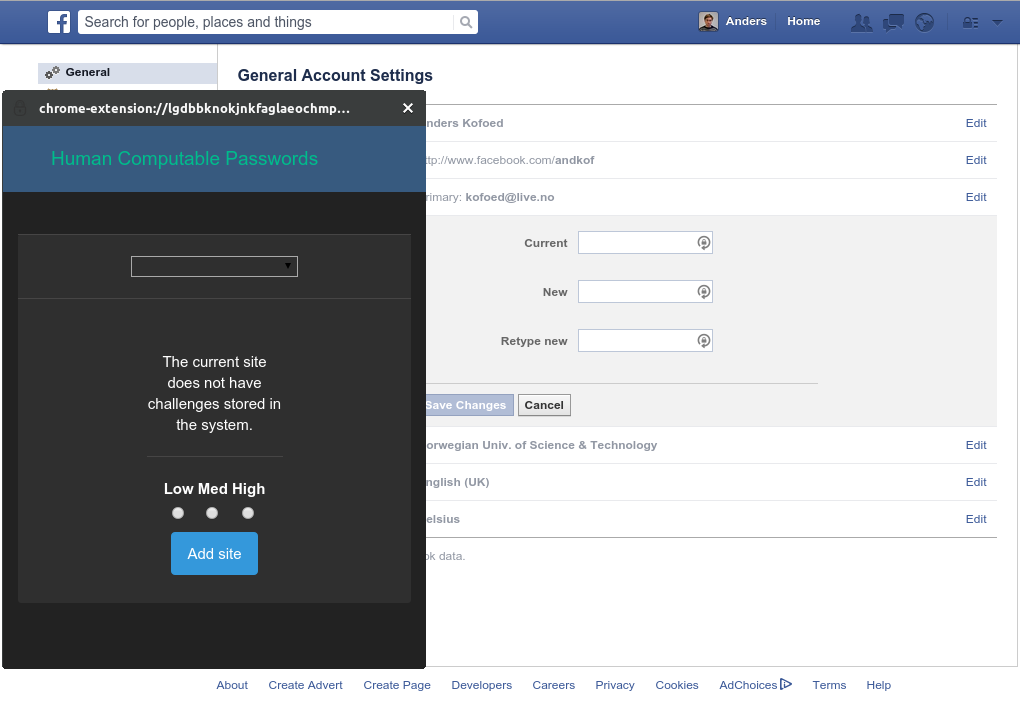
\includegraphics[width=\textwidth]{new-site-dialog2} 
    \caption{Screen as seen by the user after launching the extensions while on a page without stored challenges. After clicking the "Add site"-button, the view updates, showing the newly generate challenges. Users should then calculate the response and change the password of the site to match it. Next time the same user wants to log in to the site, they will calculate the response again as seen in figure~\ref{ch-screens}.}
    \label{launch-screen}
\end{figure}

\begin{figure}
    \centering
    \begin{subfigure}[t]{0.45\textwidth}
        \centering
        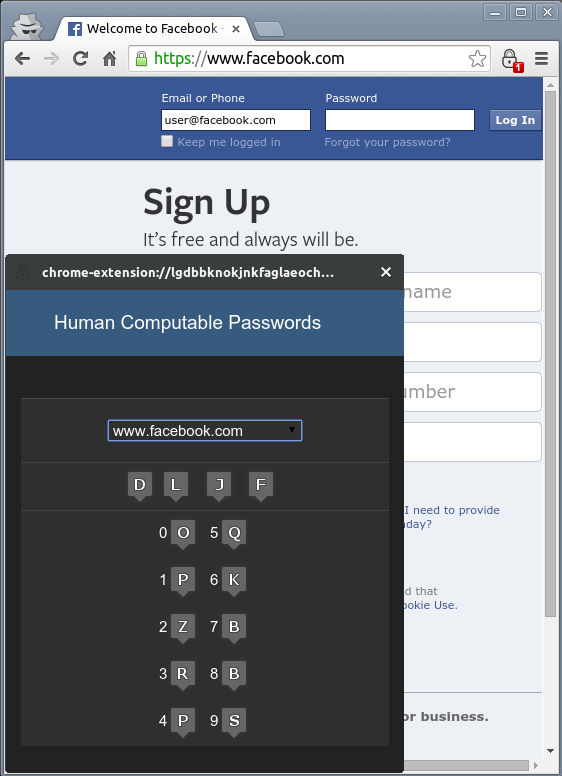
\includegraphics[width=\textwidth]{ch-screen1} 
        \caption{}
        \label{challenge-screen1}
    \end{subfigure}
    \hfill
    \begin{subfigure}[t]{0.45\textwidth}
        \centering
        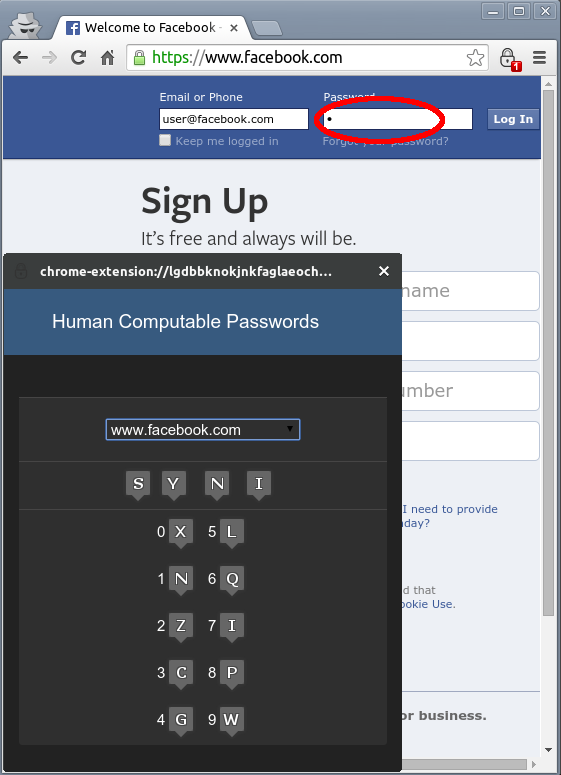
\includegraphics[width=\textwidth]{ch-screen2} 
        \caption{}
        \label{challenge-screen2}
    \end{subfigure}
    \hfill
    \begin{subfigure}[t]{0.45\textwidth}
        \centering
        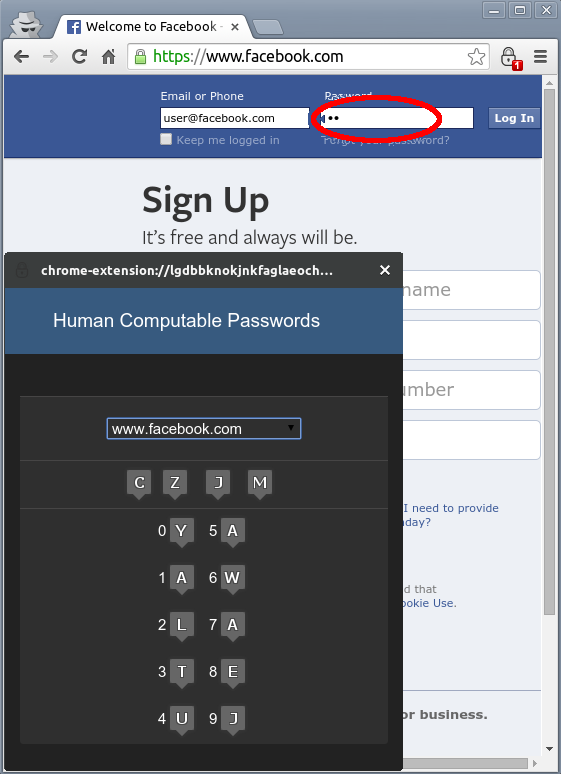
\includegraphics[width=\textwidth]{ch-screen3} 
        \caption{}
        \label{challenge-screen3}
    \end{subfigure}
    \hfill
    \begin{subfigure}[t]{0.45\textwidth}
        \centering
        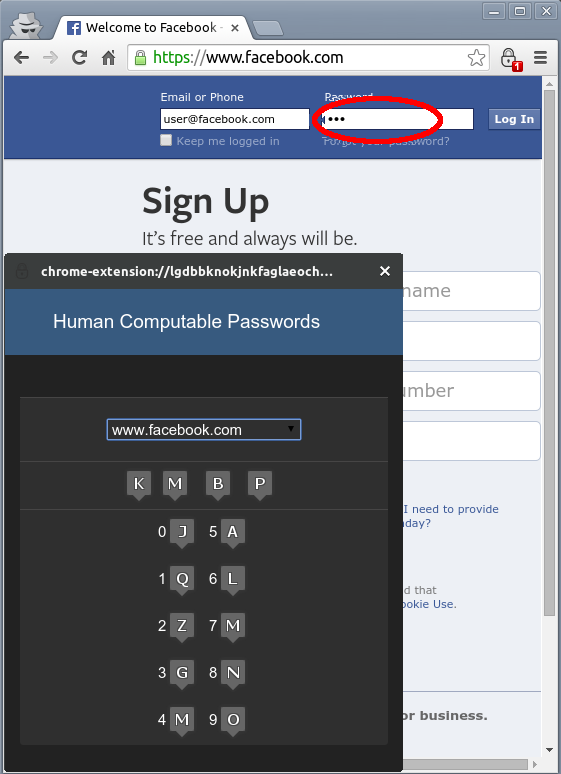
\includegraphics[width=\textwidth]{ch-screen4} 
        \caption{}
        \label{challenge-screen4}
    \end{subfigure}
    \caption{Challenge screens as seen by the user while entering password. The challenges update when the user enter a new character in the password field.}
    \label{ch-screens}
\end{figure}



\subsubsection{Data flow}\label{data-flow}
Figure \ref{flow-chart} illustrates the life cycle of the application. When the user visit a site, an event is triggered and caught by the content script, which in turn informs the controller about the newly loaded site. The controller then tries to load challenges for that site from the storage; if there is a record, the view is updated with the first challenge, if not the ``add new''-dialog is loaded. Next event is triggered when the user enters a character in the password field, on receiving notice from the content script the controller updates the view with a new challenge depending on the length of the password. This then goes on until the user has entered the entire password, eventually closing the extension panel.
%\begin{figure}
%    \centering
%    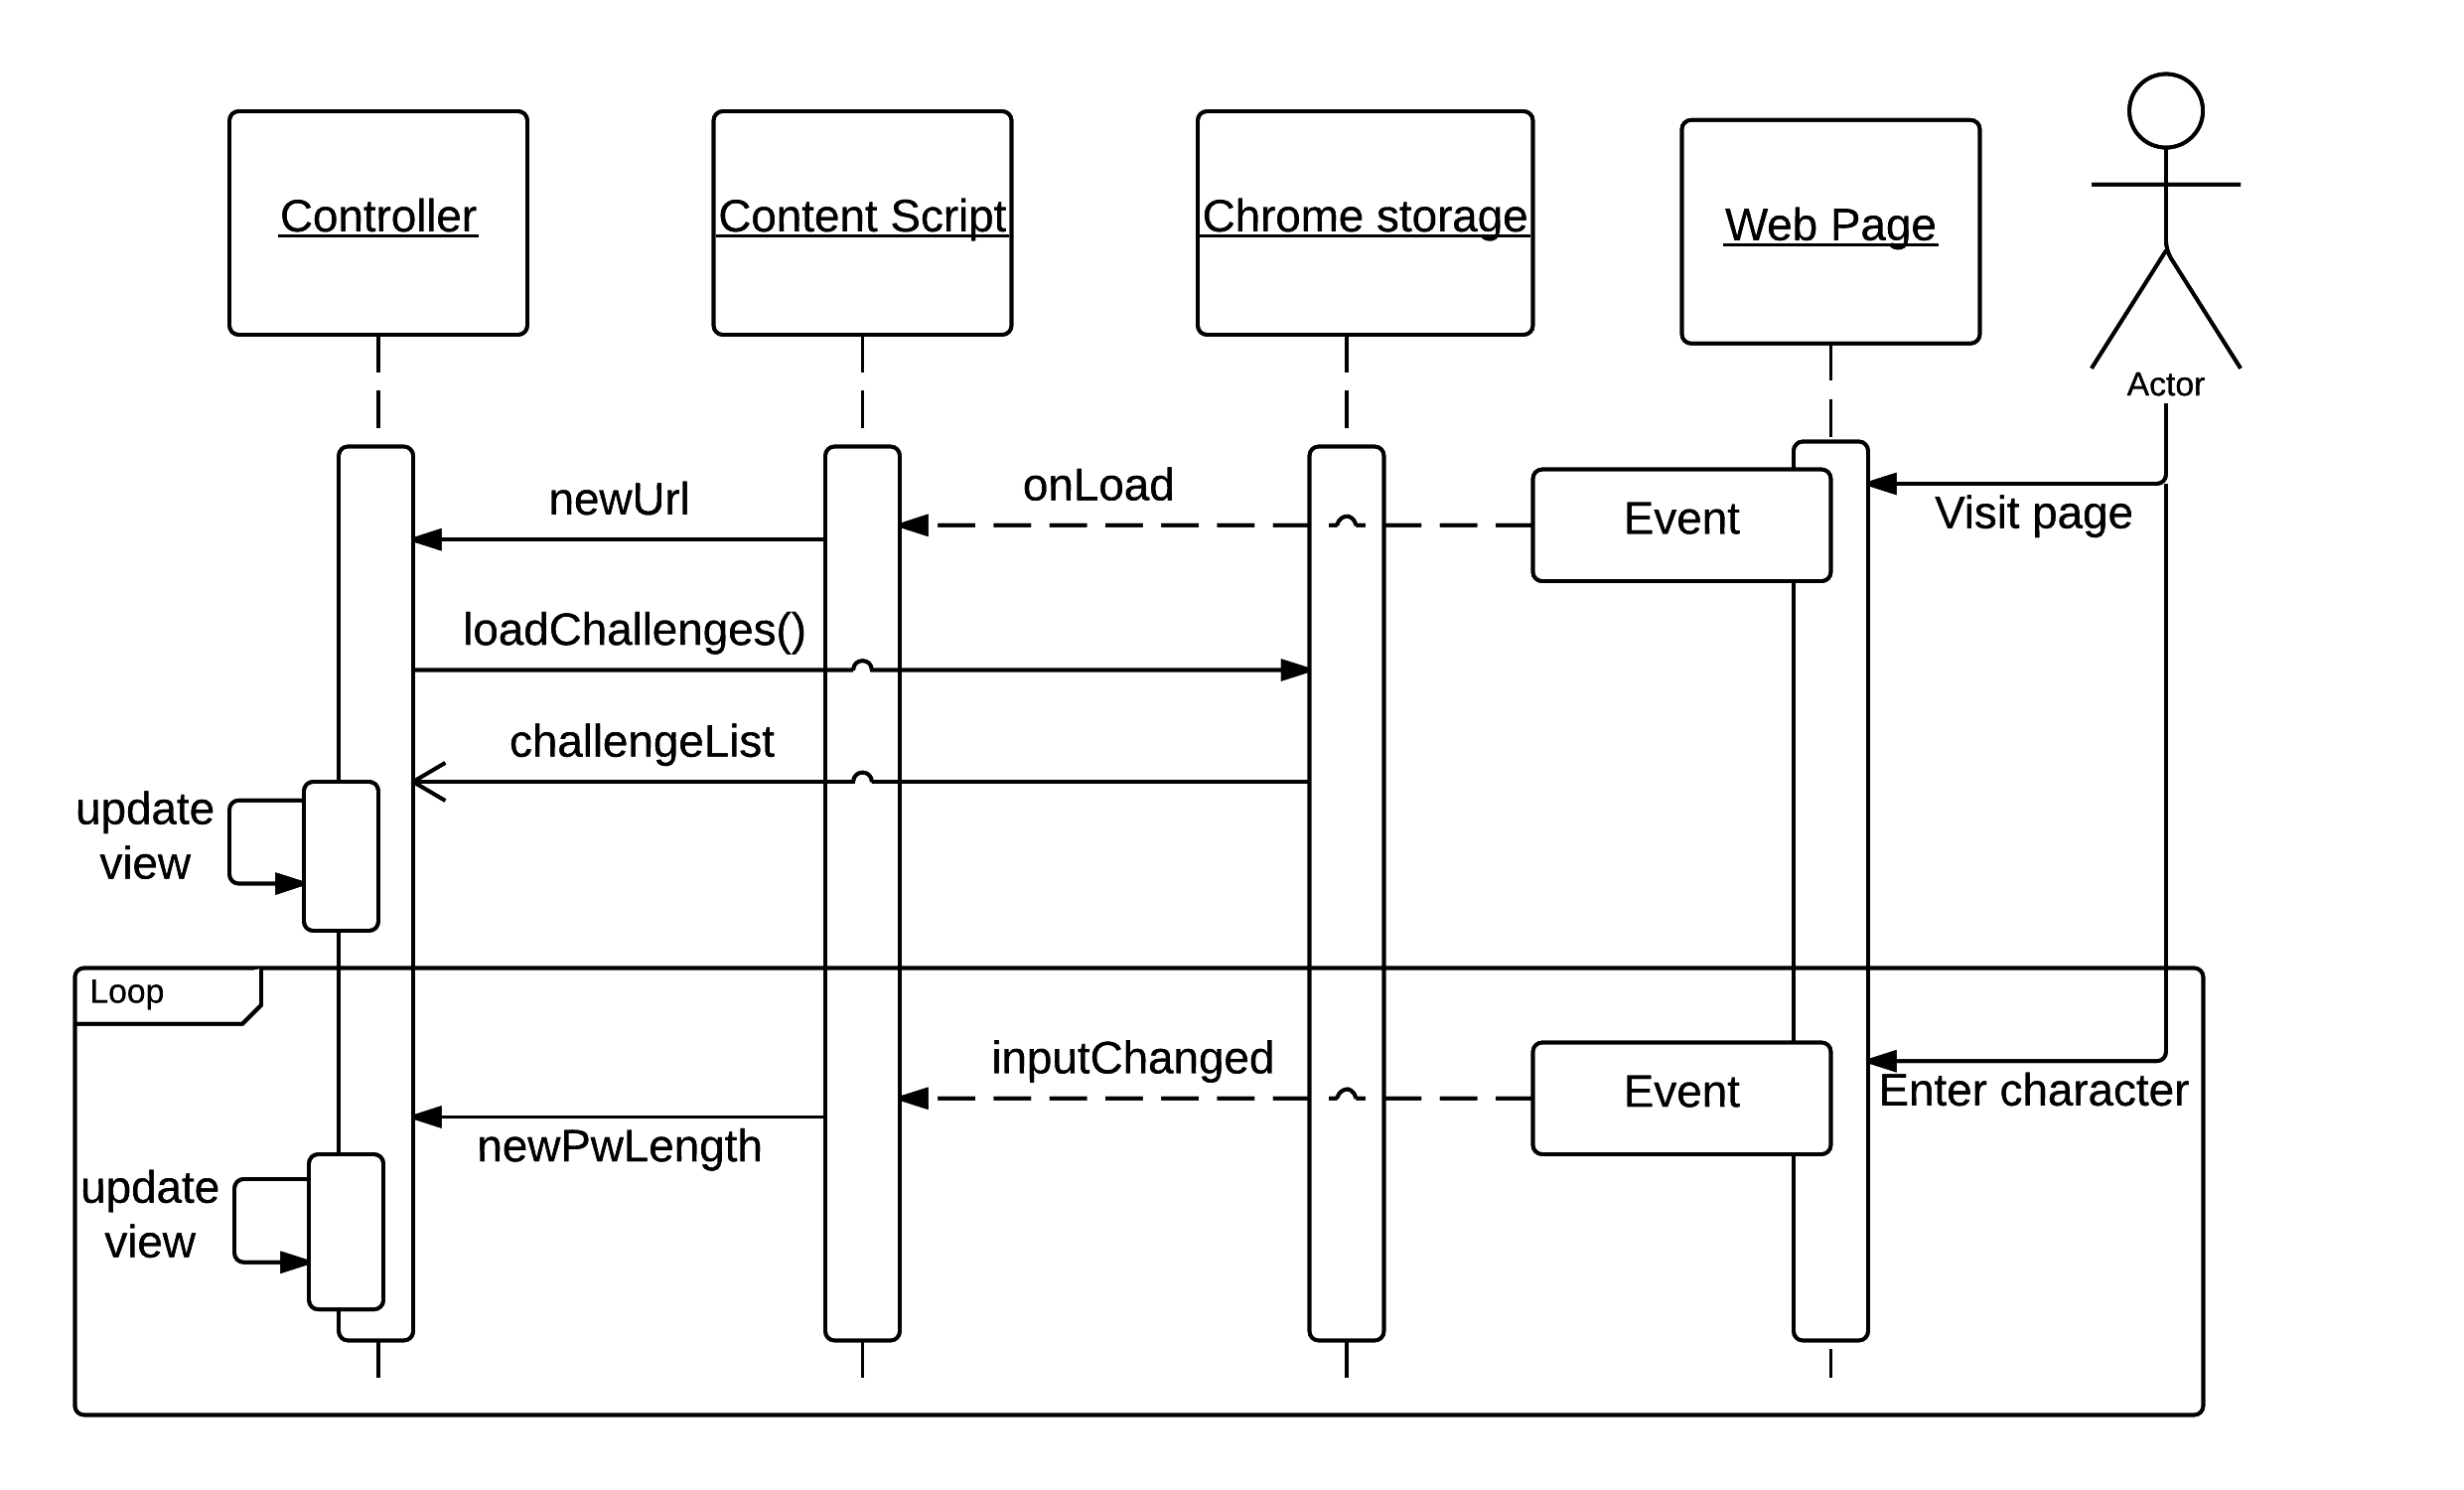
\includegraphics[width=\textwidth]{flow-chart} 
%    \caption{Sequence diagram showing the flow in the system when a page is loaded and characters typed in a password field.}
%    \label{flow-chart}
%\end{figure}


\renewcommand{\newthread}[3][0.2]{
    \newinst[#1]{#2}{#3}
    \stepcounter{threadnum}
    \node[below of=inst\theinstnum,node distance=0.8cm] (thread\thethreadnum) {};
    \tikzstyle{threadcolor\thethreadnum}=[fill=gray!30]
    \tikzstyle{instcolor#2}=[fill=gray!30]

}

\begin{figure}
    \centering    
\begin{sequencediagram}
    \newthread{ctrl}{Controller}
    \newthread[1]{cs}{Content Script}
    \newinst[1]{store}{Chrome Storage}
    \newthread[1]{page}{Web Page}
    \newthread{u}{User}

    \mess{u}{Visit page}{page}{}
        \mess{page}{pageLoadEvent}{cs}{}
            \mess{cs}{newUrl}{ctrl}
            \begin{call}{ctrl}{\hspace{3cm}loadChallenges()}{store}{}
            \end{call}

            \begin{callself}{ctrl}{update view}{}
            \end{callself}

    
    \begin{sdblock}{Loop}{}
        \mess{u}{New char}{page}{}
            \mess{page}{inputChangedEvent}{cs}{}
                \mess{cs}{newPwLength}{ctrl}
                \begin{callself}{ctrl}{update view}{}
                \end{callself}

    \end{sdblock}

\end{sequencediagram}
\caption{Sequence diagram showing the flow in the system when a page is loaded and characters typed in a password field.}
\label{flow-chart}
\end{figure}











\subsection{Discussion}
The approach of this project when designing the HCP extension was to make a clean and intuitive application, making the password management scheme feasible to use. The extension does not require any user interaction, except from when adding new sites, this was done so the user could focus on doing the calculation correctly without having to keep track of the challenges. The scheme itself is also quit complicated so it is important for the user to focus on as few operations as possible. (The simplest approach would be to have a ``next''-button for the user to click between every character calculated.)
\par The choice of a browser extension was done with the same mind set, making the application helpful and not distracting. It should be easy to start using the application, requiring as little configuration and managing as possible. The design and construction makes it so that the only configuration required is the changing of passwords when adding sites, which essentially can not be circumvent. Panels is another very useful feature, since the panels float on top of the other browser windows and keep focus while typing. Without panels the user would have to switch between windows when calculating a character and typing it in the password field, which would be a huge drawback both in terms of time and usability. 
\par One apparent problem with using extensions is that they are not supported in mobile browsers, and probably will never be\footnote{Multidevice FAQ - \url{https://developer.chrome.com/multidevice/faq}}. The solution to this would be to make an additional application for mobile, and sync the data to another service available on mobile as well. This could be done quite easily since the data is stored as text, the only change needed would be to substitute the storage module with some other cloud storage service. The problem if the application was built for mobile would be the lack of space to display challenges while typing the password. 
\par As mentioned in 
\par The decision to make a browser extension was made on behalf of the mentioned pros and cons, with the most important parameter being disturbance. Only extensions allow a seamless, non-interfering user interface. The other options, namely web application and mobile application, would require switching between windows or at least switching of focus, as well as requiring the user to manually chose the correct site and browse through the different challenges. This is all done automatically with the construction presented in this chapter. The main goal of the design was to include the least amount of unnecessary features, with a clean and unobstructive interface. A summary of the strengths of the chosen design is listed next.

\begin{itemize}
    \item Easy to use, require little to no user interaction after configuration.
    \item Panel that stay on top while entering the password allows for quick and easy calculation without stopping to update and manage challenges.
    \item Chrome.storage.sync automatically synchronize the stored challenges to the users Google account allowing persistent usage across devices and accounts.
    \item All data is stored as text strings, this makes it easy to integrate with other services in the future. Users could also store the challenges elsewhere if need be, e.g. as text locally or even print the challenges on paper in the extreme case.
\end{itemize}






